\documentclass[10pt,onecolumn]{lab}


% All KJN's macros and goodies (some shameless borrowing from SPL)
\usepackage{KJN}


%\usepackage[hyphens]{url}

%
% PDF Info
%
\ifpdf
\pdfinfo{
/Title (SOFTWARE ENGINEERING PROJECT: STUDENTS MARKS/RECORDS MANAGEMENT SOFTWARE)
/Author (Khosa Masana (559990), Sanele Gcaba(459380), Tshegofatso Misapitso (600313), Londiwe Ngema (448871) )
/ModDate (D:200510121530)
/Subject (ELEN417/455 Paper Format, 2005)
/Keywords (ELEN417, ELEN455, paper, instructions, style guidelines, laboratory project)
}
\fi

%%%%%%%%%%%%%%%%%%%%%%%%%%%%%%%%%%%%%%%%%%%%%%%%%%%%%%%%%%%%%%%%%%%%%%%%%%%%%%%
\begin{document}

\begin{titlepage}

\newcommand{\HRule}{\rule{\linewidth}{0.5mm}} % Defines a new command for the horizontal lines, change thickness here

\center % Center everything on the page
{\small School$\;$of$\;$Electrical$\;$and$\;$Information$\;$Engineering,$\;$University of$\;$the$\;$Witwatersrand,$\;$Private$\;$Bag$\;$3,$\;$2050,$\;$Johannesburg,$\;$South$\;$Africa}\\[1.5cm] % Name of your university/college

\textsc{ELEN 4009 - Software Engineering}\\[0.5cm] % Major heading such as course name

\HRule \\[0.4cm]
{ \large \bfseries Student Marks/Records Management Software - Requirements Gathering}\\[0.4cm] % Title of your document
\HRule \\[1.5cm]

 \large

\textbf{Project Team :}
Khosa$\;$Masana$\;$(559990),
Sanele$\;$Gcaba$\;$(459380),
Tshegofatso$\;$Misapitso$\;$(600313) and
Londiwe$\;$Ngema$\;$(448871)


{\large \today}\\[3cm] % Date, change the \today to a set date if you want to be precise

%\includegraphics{Logo}\\[1cm] % Include a department/university logo - this will require the graphicx package

\vfill % Fill the rest of the page with whitespace

\end{titlepage}

\pagestyle{plain}.
\pagenumbering{roman} 
\tableofcontents 
\newpage

\section{Project Scope}
\begin{itemize}

\item There are three basic users of the system - Students, Course coordinators and School administrator.
\item The primary function of the application is to allow students and staff  to log-in using their details (Student/Staff number and password) and be able to access and view student records, the records include student marks for all forms of assessments for all courses registered for. 
\item The system database stores user profiles and student marks records. Marks records are retained for a period of 10 yrs.
\item The software program should have domains assigned, i.e. each user can be able to access relevant  information and they are allowed to view/edit/add based on what their recognised  domain.
\item  The system would be accessed online via a Browser and/or a Smart-phone App.

\end{itemize}

Below is a list of privileges per user as specified on the project brief \cite{ref9}.

\textbf{The Course Coordinator should be able to:-}
\begin{itemize}
\item Register himself/herself.
\item Add various assessment method for the course and weighting for each assessment.
\item Enter student marks on a user-friendly interface.
\item Display or print out the table of students and their marks.
\item Generate a summary statistics of the performance of the students - maximum, minimum, average, standard deviation or variants of each assessment.  
\item View projected pass rate based on the assessment marks accumulated students in class.
\end{itemize}

\textbf{The School Administrator should be able to:-}
\begin{itemize}
\item Register himself/herself.
\item Display or print out table of students and their marks.
\item Generate a summary statistics of the performance f the students. 
\item Generate a comparative chart of the assessment marks of selected courses being taken by students of a particular group. 
\item Histogram of assessment marks of all courses taken a specific student.   
\item Any recorded offences (e.g. plagiarism) for a student.
\item The performances in the same course across different years may be compared.
\end{itemize}

\textbf{The Student should be able to:-}
\begin{itemize}
\item Register himself/herself.
\item Display assessment marks for a course and statistics for that assessment.
\item Display assessment marks for all the courses  
\item Based on current assessment marks, give what performance goals are needed to pass the course.
\end{itemize}

\section{List of Definitions and abbreviations}

\subsubsection{Definitions}
\begin{center}
    \begin{tabular}{ | p{3cm} | p{9cm} |}
\hline
\textbf{Term}& \textbf{Definition}\\ \hline
 Database & A collection of records stored within the system \\ \hline
 Table & A collection of related data consisting of columns and rows \\ \hline   
     \end{tabular}
\end{center}

\subsection{Abbreviations}~\\

\textbf{SMMS} - Student Marks/record management system

\textbf{HTTP} - Hypertext Transfer Protocol

\textbf{HTML} - HyperText Markup Language

\textbf{RDBMS} - Relational Database Management System

\textbf{SQL} - Structured Query Language

%%%%%%%%%%%%%%%%%%%%%%%%%%%%%%%%%%%%%%%%%%%%%%%%%%%%%%%%%%%%%%%%%%%%%%%%%%%%%%%  

\section{Expanded Description of the project}

The software system will follow a Two-Tier Architecture due to its ease of use and maintainability as compared to a Three-Tier Architecture. However, the performance of a Two-Tier Architecture slows down with an increase in users \cite{ref3}, hence a Three-Tier Architecture will be implemented with an increase of the number of users. Figure 1 below shows the Two-Tier Architecture.   
\begin{center}
\begin{figure}[h]
\centering
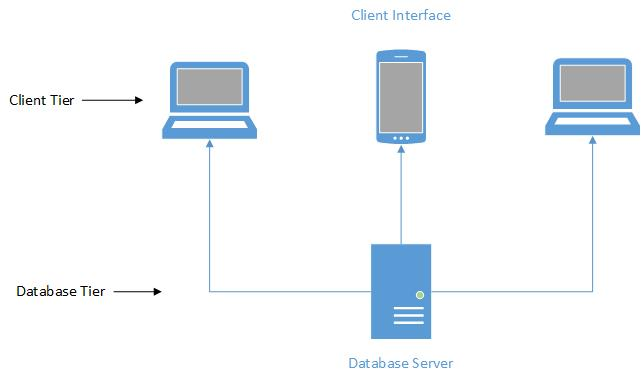
\includegraphics[width=10cm]{Two-Tier}
\caption{Two-Tier Software Architecture}
\end{figure}
\end{center}


A Two-Tier Architecture is a software architecture where the interface runs on client and the data layer is stored on a server\cite{ref4}.

\section{Responsibilities}

Masana Khosa and Londiwe Ngema are responsible for the front end, they designed the website page and the interfaces for the individual users. They also created domains to ensure that the user only has access to what they need.

Sanele Gcaba and Tshegofatso Misapitso are responsible for the back end that is the database. The next step is to do the querying logic to link the back and front ends. The program is now able to log the registered users in and out based on the information from the database. Different interfaces can now be called upon for different users, i.e different interfaces for the school administrator, course co-ordinator and the students.

\section{The current prototype}

\subsection{Front-End}
The current prototype allows users to log in and they are redirected to the different pages based on the scope above. Since there are types of users with different privileges, they are distinguished using a domain. A student cannot log on the system as a stuff member and vice versa. When a user logs out they are directed to the home page.

\subsection{Back-End}
The developed Back-End constitute of a LAMP web server, this is hosted within a PC and accessible using a local host of a machine. The server that hosts the database was created using PHPmyadmin. The Back-end has achieved creating a database for users, this database has a Username, Password and Domain. The back-end team has been able ensure a link between the front end interface and the login database. 

Figure below shows the user database design.

\begin{center}
\begin{figure}[h]
\centering
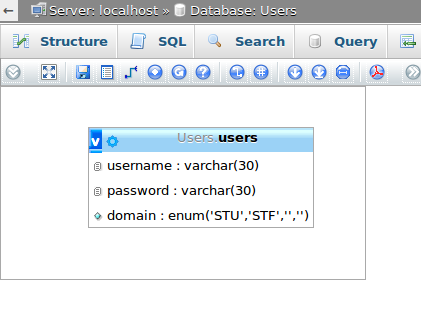
\includegraphics[width=10cm]{Users}
\caption{User Database}
\end{figure}
\end{center}
     
Additionally a student record Database was created and a figure below shows a structure for the database

\begin{center}
\begin{figure}[h]
\centering
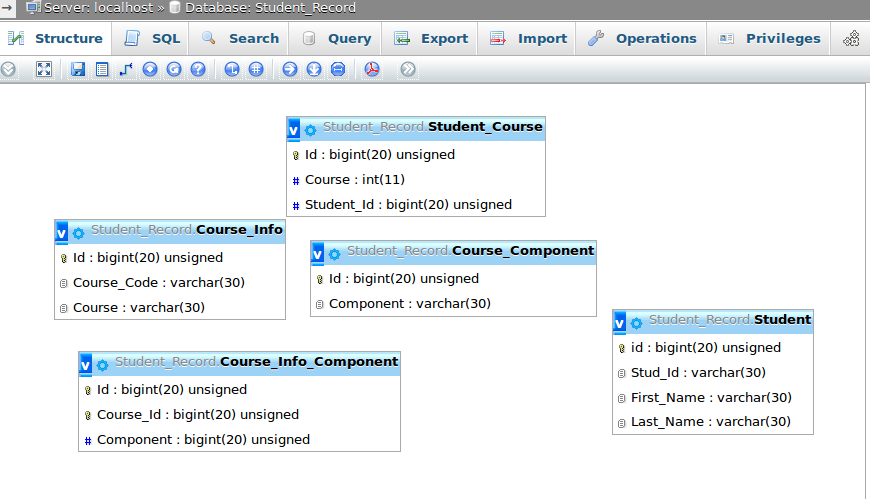
\includegraphics[width=10cm]{StudentRecord}
\caption{Student Record Database}
\end{figure}
\end{center}
  
\newpage


 
\vfill
%\nocite{*}
\bibliographystyle{witseie}
\bibliography{sample}

%{\tiny \vfill \hfill \today \hspace{5mm} witseie-paper-2003.\TeX}

\end{document}

" vim: ts=4
" vim: tw=78
" vim: autoindent
" vim: shiftwidth=4
